\section{总体分析}

四个问题围绕“药材烘干”这一物理过程逐层递进，本质都是求解圆柱药材内部的\textbf{温度场}与\textbf{水分浓度场}，其核心是\textbf{非稳态热传导方程}与\textbf{水分扩散方程}的耦合求解，区别在于物性参数、边界条件与求解目标的不同。

从物理机理看，热风烘干涉及两类输运过程：其一为\textbf{热量输运}，热空气通过对流将热量传给药材表面，再经热传导向中心渗透，使药材温度升高；其二为\textbf{水分输运}，表面水分在浓度差驱动下向空气中蒸发，内部水分因浓度梯度向表面扩散补充。二者通过物性参数耦合——密度 $\rho$、比热容 $c_p$、导热系数 $k$ 与水分扩散系数 $D$ 均随含水率 $C$ 变化（扩散系数 $D$ 还强烈依赖温度 $T$），因此需联立求解。

在几何处理上，药材长径比为 $25/4=6.25$，远大于 1，端面效应可忽略，且题目要求给出“到药材中心的距离”处的分布，故可采用\textbf{一维径向（长圆柱近似）}模型，将问题降维为径向坐标 $r$ 上的偏微分方程组，显著降低计算复杂度。四个问题的递进关系如下：

\begin{itemize}
	\item \textbf{问题一（预热平衡阶段）}：烘房温湿度随时间变化（附件 1），物性为常数（附录 2），求解短时段（30 min）内的温度与水分分布，属于瞬态问题的“基础模型”。
	\item \textbf{问题二（整个烘干过程）}：物性随含水率、温度变化（附录 3），环境由预热段过渡到恒温段，建立覆盖全过程的变物性模型，考察 3 h 内的演化规律。
	\item \textbf{问题三（干燥时间）}：在问题二模型基础上，引入“处处含水率 $<0.15$ kg/kg”的判据，将问题转化为确定模型运行至该判据满足的终止时刻。
	\item \textbf{问题四（尺寸收缩）}：进一步考虑失水收缩引起的半径变化（附件 2），将固定区域扩展为\textbf{移动边界}问题，结合附录 4 物性求解真实工况下的干燥时长。
\end{itemize}

在求解方法上，一维径向扩散方程可统一写成守恒形式，采用\textbf{控制体积法}在空间上离散，时间方向采用二阶精度的\textbf{Crank--Nicolson 隐式格式}，既保证无条件稳定，又能以较大时间步长获得高精度；传热与传质之间的非线性耦合通过每个时间步内的\textbf{固定点迭代}处理。该方法对四个问题统一适用，仅需更换物性公式与边界条件。总体建模框架如图~\ref{fig:geometry} 所示。

\begin{figure}[htbp]
	\centering
	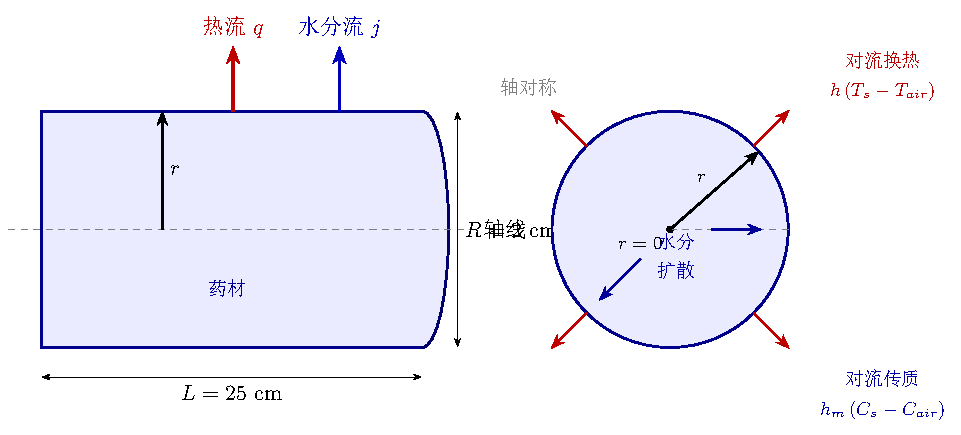
\includegraphics[width=0.78\textwidth]{texfile/figures/fig_geometry.pdf}
	\caption{圆柱药材传热传质示意图（左：侧视图；右：横截面）}
	\label{fig:geometry}
\end{figure}
